\documentclass[final]{beamer}
% ====================
% Packages
% ====================
\usepackage{url}
\usepackage[T1]{fontenc}
\usepackage{lmodern}
\usepackage[orientation=portrait,size=a0,scale=1.00]{beamerposter}
\usetheme{gemini}
\usecolortheme{UBI}
\usepackage{graphicx}
\usepackage{booktabs}
\usepackage{tikz}
\usepackage[portuguese]{babel}
\usepackage{pgfplots}
\usepackage{subfigure}
\pgfplotsset{compat=1.14}
\usepackage{anyfontsize}
\usepackage{xcolor}
\usepackage[skip=2pt,font=normalsize]{subcaption}
\usepackage{adjustbox}
\usepackage{tikz}
\usetikzlibrary{shapes.geometric, arrows}
% ====================
% Lengths
% ====================
% If you have N columns, choose \sepwidth and \colwidth such that
% (N+1)*\sepwidth + N*\colwidth = \paperwidth
\newlength{\sepwidth}
\newlength{\colwidth}
\setlength{\sepwidth}{0.025\paperwidth}
\setlength{\colwidth}{0.45\paperwidth}
\newcommand{\separatorcolumn}{\begin{column}{\sepwidth}\end{column}}
% ====================
% Title
% ====================
\title{Queda de uma mola ideal suspensa com massas distribuídas regularmente}
\author{José Amoreira \inst{1,2,3} \and João Santos \inst{2} \and João Esteves \inst{2}}
\institute[]{\inst{1} Laboratório de Instrumentação e Física Experimental de Partículas \and  \inst{2}Universidade da Beira Interior  \samelineand \inst{3} Centro de Matemática e Aplicações}
% ====================
% Footer (optional)
% ====================
\footercontent{
  Física 2024 \hfill
  UBI - Departamento de Física}
% (can be left out to remove footer)
% ====================
% Logo (optional)
% ====================
% use this to include logos on the left and/or right side of the header:
%\logoright{
\includegraphics[scale=1.5]{logos/DF2.png}}
\logoleft{
\includegraphics[scale=1.5]{logos/DF2.png}}
% ====================
% Body
% ====================
\begin{document}

\begin{frame}[t]
\begin{columns}[t]
\separatorcolumn

\begin{column}{\colwidth}

% ----------------------------------
% Abstract
% ----------------------------------
  \begin{exampleblock}{Motivação/Introdução}
Vários vídeos disponíveis na plataforma YouTube mostram a queda de uma mola
elástica a partir de uma situação de repouso estático em que ela se encontra na
vertical, suspensa de uma das suas extremidades. Estes vídeos são interessantes
poque mostram a extremidade inferior da mola como que a aguardar que a
extremidade superior a atinja, antes de começar o seu movimento de queda
propriamente dito. 

A explicação deste comportamento é dada pela teoria da elasticidade de um meio
contínuo. A onda de deformação gerada na extremidade superior da mola quando é
solta propaga-se longitudinalmente com uma velocidade finita, e só quando atinge
a extremidade inferior, alterando aí o estado de deformação inicial, se altera o
equilíbrio de forças (peso e força elástica) que mantinham esta extremidade em
repouso.

Claramente, o modelo elementar de mola ideal, em que se despreza a sua massa, é
insuficiente para enquadrar esta explicação, uma vez que não tendo massa, (3)~a
mola não fica sujeita à gravidade, ou seja, não cai e (1)~a sua deformação é
sempre uniforme, pelo que a força sobre a extremidade inferior altera-se
instantaneamente assim que a extremidade superior inicia a sua queda. 

Com este trabalho, tentou-se descrever o movimento de queda das molas reais
usando o modelo de mola ideal, com massas iguais distribuídas uniformemente
sobre o seu comprimento.
  \end{exampleblock}
  

\begin{block}{Formalismo}
    Aplicando a segunda lei de Newton a este formalismo, ficamos com:
    \begin{align*}
        \ddot x_0 &=-Ng+\omega^2(x_1-x_0)\\[1cm] 
        \ddot x_i &= \omega^2(x_{i-1}-2x_i+x_{i+1}),\qquad i=1, \ldots, N-2\\[1cm]
         \ddot x_{N-1} &=\omega^2(x_{N-2}-x_{N-1})
    \end{align*}    
\end{block}

\begin{block}{Procedimento experimental}
   Foi observada e gravada a queda do conjunto mola e bola para compreender o seu comportamento. O experimento foi realizado de duas maneiras diferentes, com duas bolas e uma mola, e com três bolas, dividindo a mola ao meio. Ambas as execuções foram gravadas em câmara lenta, a uma taxa de 120 frames por segundo, e posteriormente analisadas usando o software Tracker.
    % This flow chart is created by the author

% adjustbox is used to limit the figure inside the page
% -- means normal arrow
%  -| horizontal followed by the vertical arrow
%  |- vertical followed by the horizontal arrow


\begin{figure}

    \begin{center}
        \begin{adjustbox}{max height=\textheight, center, width=0.8\textwidth}
            \begin{tikzpicture}
\tikzstyle{spring}=[thick,decorate,decoration={aspect=.5, segment length=5, amplitude=2.5mm,coil, post length=0, pre length=0}]
   % \draw[pattern={north east lines}] (-1,5.2) rectangle (1,5.4);
    \draw [spring] (0,0) -- (0,-5);
    \node[] at (0,-8) {$(a)$};
    \draw [fill=white] (0,0) circle (.5) node[draw=none,inner sep = 0,scale=2,text=black]{$m$};
    \draw [fill=white] (0,-5) circle (.5) node[draw=none,inner sep = 0,scale=2,text=black]{$m$};
%________________________________________________________________%
\tikzstyle{spring}=[thick,decorate,decoration={aspect=.5, segment length=6, amplitude=2.5mm,coil, post length=0, pre length=0}]
    \draw [spring] (3,0) -- (3,-3);
   \draw [fill=white] (3,0) circle (.5) node[draw=none,inner sep = 0,scale=2,text=black]{$m$};
    \tikzstyle{spring}=[thick,decorate,decoration={aspect=.5, segment length=6, amplitude=2.5mm,coil, post length=0, pre length=0}]
    \draw [spring] (3,-3) -- (3,-7);
    \draw [fill=white] (3,-3) circle (.5) node[draw=none,inner sep = 0,scale=2,text=black]{$m$};
    \draw [fill=white] (3,-7) circle (.5) node[draw=none,inner sep = 0,scale=2,text=black]{$m$};
    \node[] at (3,-8) {$(b)$};
            \end{tikzpicture}
        \end{adjustbox}
    \end{center}
    \caption{Caption for flowchart.}
    \label{fig:figure1}
\end{figure}
 A constante elástica tanto para a mola completa quanto para a metade da mola foi determinada por meio de outro experimento. Com esses resultados em mãos, os valores teóricos foram calculados utilizando o Python e comparados com os resultados experimentais obtidos pelo Tracker. \emph{(mais informação no código QR)}
\end{block}

% -------------------------------
% Section: Descriptive Statistics
% -------------------------------


\end{column}

\separatorcolumn

\begin{column}{\colwidth}

% -------------------------------
% Section: Results and discussion
% -------------------------------

\begin{block}{Resultados}
    
    Após realizar o procedimento todo explicado no bloco anterior, podemos então observar os resultados:
    \begin{figure}
    \centering
    \subfigure[]{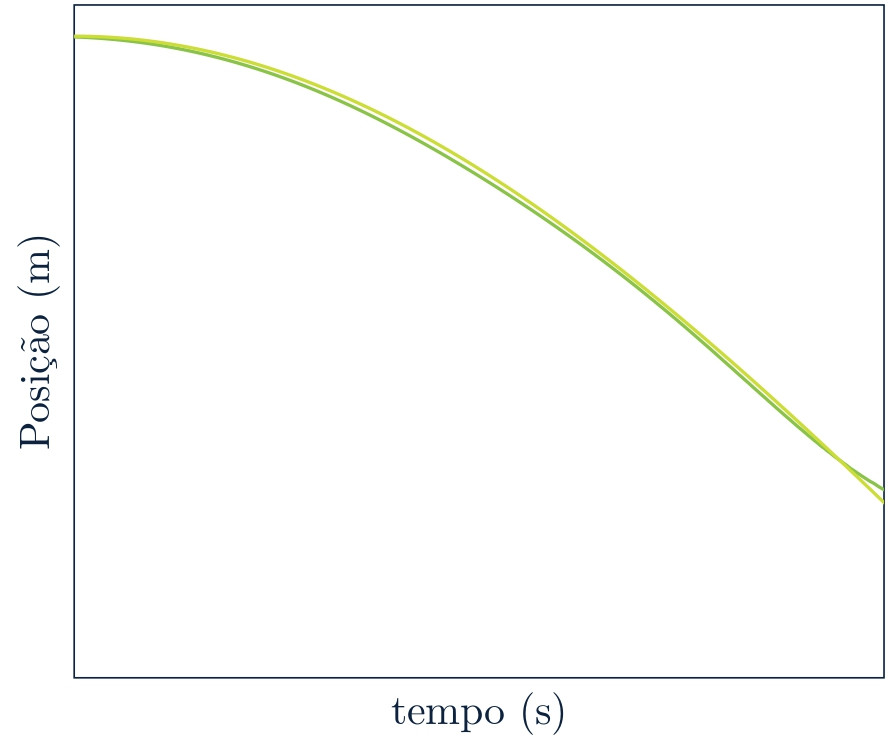
\includegraphics[width=0.3\columnwidth]{images/1.jpg}} 
    \subfigure[]{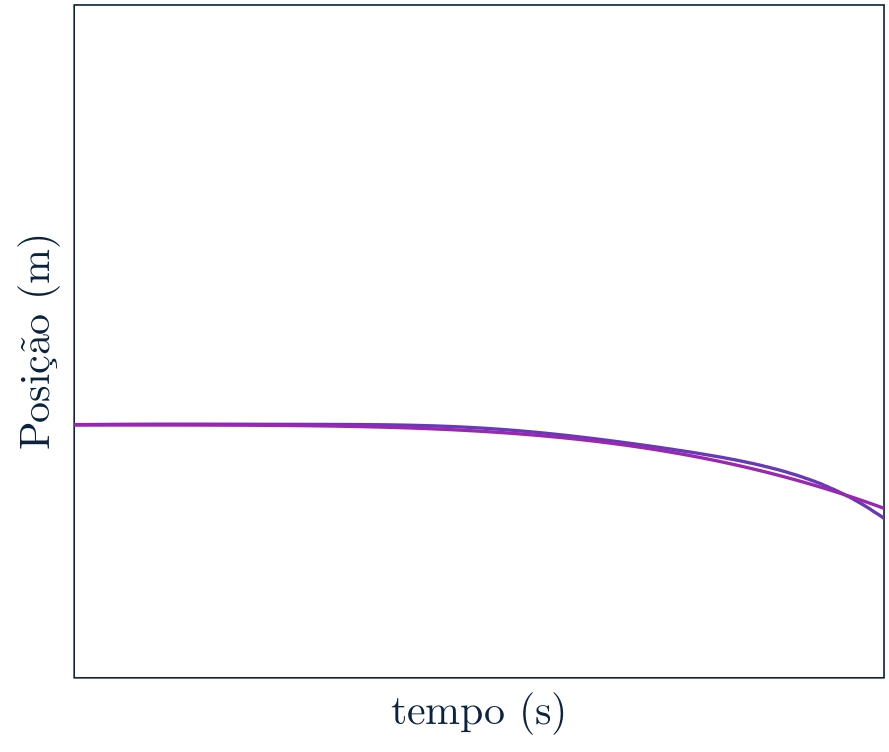
\includegraphics[width=0.3\columnwidth]{images/2.jpg}} 
    \subfigure[]{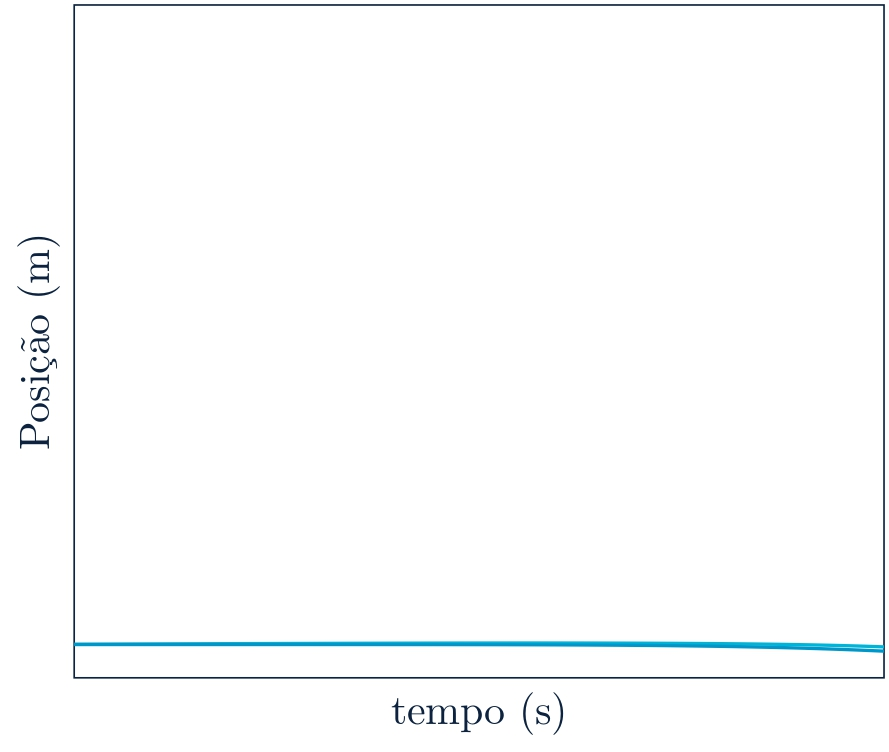
\includegraphics[width=0.3\columnwidth]{images/3.jpg}}
    \caption{(a) Resultados Bola 1 (b) Resultados Bola 2  (c) Resultados Bola 3}
    \label{fig:foobar}
\end{figure}
    E, observando as três no mesmo gráfico
   \begin{figure}
   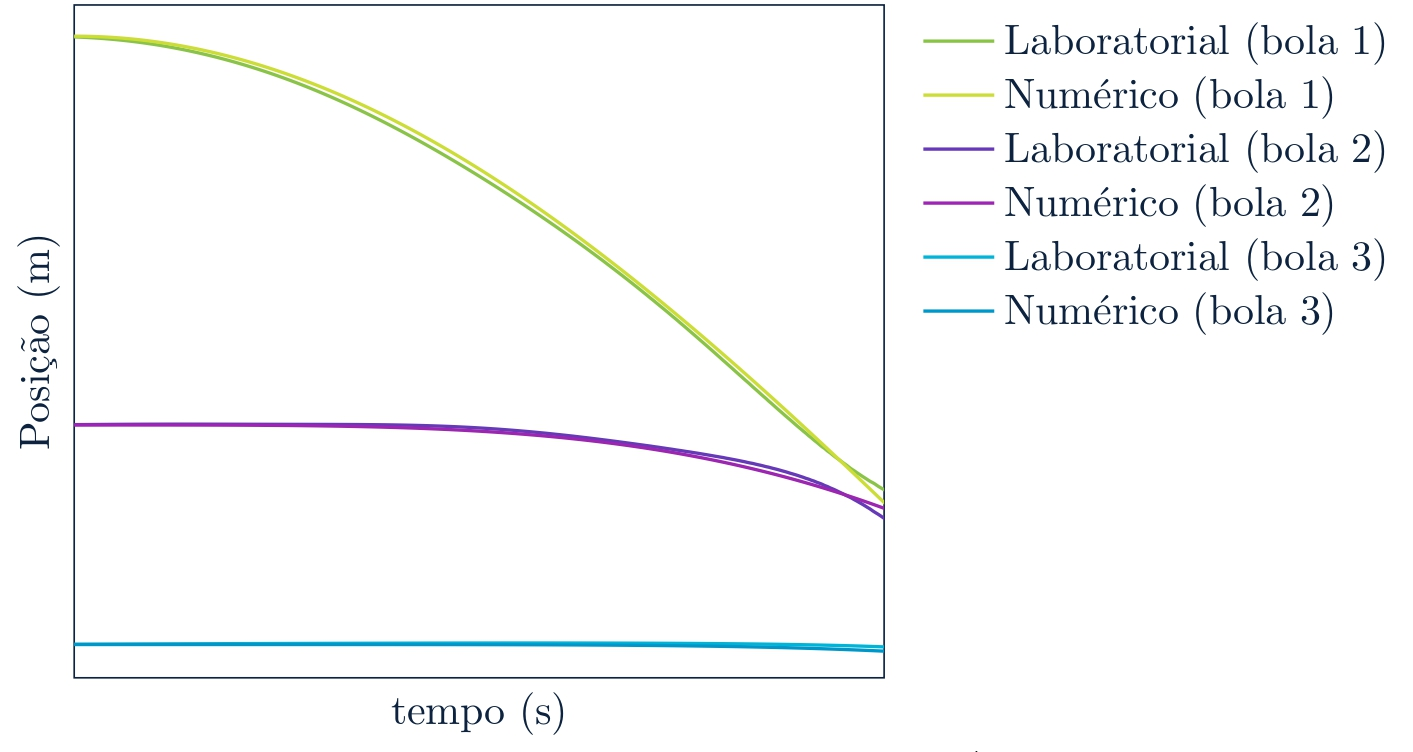
\includegraphics[width=.5\columnwidth]{images/4v2.jpg}
   \caption{Comparação dos resultados experimentais e numéricos.}
   \end{figure}
\end{block}

% -------------------------------
% Section: Conclusions
% -------------------------------
   \begin{exampleblock}{Conclusões}
    \begin{itemize}
      \item Sed et augue accumsan nibh ullamcorper accumsanam dictum urna tortor, ut pretium leo eleifend.  
      \item Donec suscipit, urna quis tempus consectetur, quam est placerat ante, et scelerisque metus velit. 
      \item Nam dictum urna tortor, ut pretium leo eleifend efficitur.
      \item Praesent blandit faucibus quam, et tincidunt mauris sagittis eget 2.2\%.
      \item Dolor sit amet, consectetur adipiscing elit. Mauris in nulla ultricies suscipit.
    \end{itemize}
  \end{exampleblock}


  \begin{block}{Referencias}

    \nocite{*}
    \footnotesize{\bibliographystyle{plainurl}\bibliography{poster}}

  \end{block}

% -------------------------------
% Section: Portfolio
% -------------------------------
  \begin{block}{Mais Informações}

    \begin{figure}[h]
    \centering
    
\includegraphics[height=8cm]{images/qrcode2.png}
    \label{fig:figure3}
\end{figure}

  \end{block}

\end{column}
\separatorcolumn



\end{columns}
\end{frame}

\end{document}
